\documentclass[tikz]{standalone}

\usepackage[T1]{fontenc}
\usepackage[english]{babel}

\usepackage{graphicx}
\usepackage{standalone}
\usepackage{pgfplots}

\begin{document}
	\begin{tikzpicture}
		\node (image) {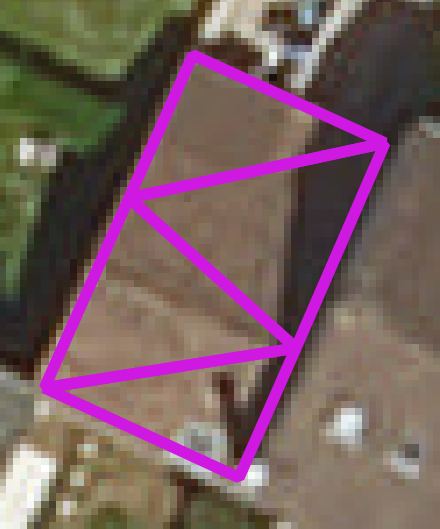
\includegraphics[width=5cm, angle=270]{images/introduction/graphical_abstract/orthoprojection}};

		\path (image) + (2.33, -1) node (segment_hist_1) {
			\resizebox{.75cm}{.75cm}{
				\begin{tikzpicture}background rectangle/.style={fill=white}, show background rectangle
					\begin{axis}[
						area style,
						axis background/.style={fill=white},
						ymin=0,
						ytick=\empty,
						xtick=\empty
					]
						\addplot+[ycomb, orange, mark=*, mark options={scale=2, fill=orange}, very thick] plot coordinates {
							(-8, 3623)
							(-7, 546)
							(-6, 159)
							(-5, 182)
							(-4, 70)
						};
					\end{axis}
				\end{tikzpicture}
			}
		};
		\path (image) + (-2.16, 1.16) node (segment_hist_2) {
			\resizebox{.75cm}{.75cm}{
				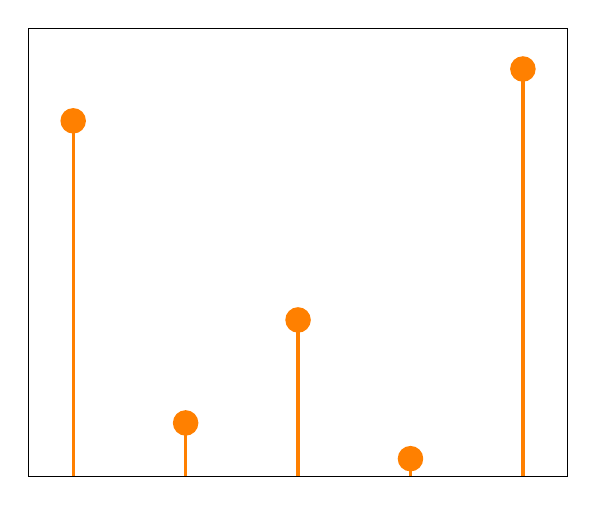
\begin{tikzpicture}background rectangle/.style={fill=white}, show background rectangle
					\begin{axis}[
						area style,
						axis background/.style={fill=white},
						ymin=0,
						ytick=\empty,
						xtick=\empty
					]
						\addplot+[ycomb, orange, mark=*, mark options={scale=2, fill=orange}, very thick] plot coordinates {
							(-8, 3623)
							(-7, 546)
							(-6, 1595)
							(-5, 182)
							(-4, 4151)
						};
					\end{axis}
				\end{tikzpicture}
			}
		};
		\path (image) + (-2.16, -.83) node (segment_hist_3) {
			\resizebox{.75cm}{.75cm}{
				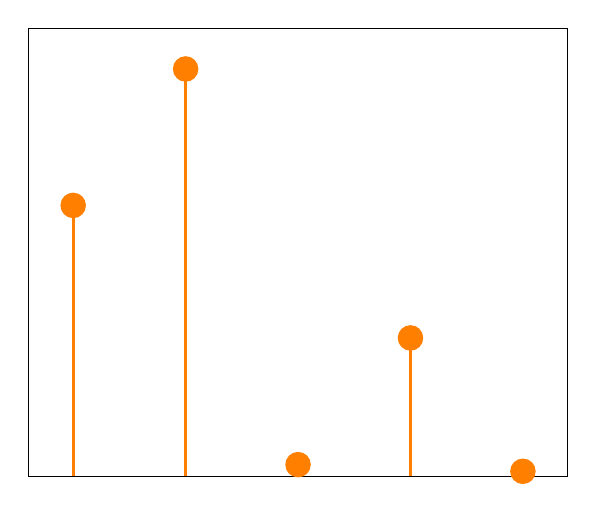
\begin{tikzpicture}background rectangle/.style={fill=white}, show background rectangle
					\begin{axis}[
						area style,
						axis background/.style={fill=white},
						ymin=0,
						ytick=\empty,
						xtick=\empty
					]
						\addplot+[ycomb, orange, mark=*, mark options={scale=2, fill=orange}, very thick] plot coordinates {
							(-8, 3623)
							(-7, 5446)
							(-6, 159)
							(-5, 1852)
							(-4, 70)
						};
					\end{axis}
				\end{tikzpicture}
			}
		};
		\path (image) + (.33, -1.66) node (segment_hist_4) {
			\resizebox{.75cm}{.75cm}{
				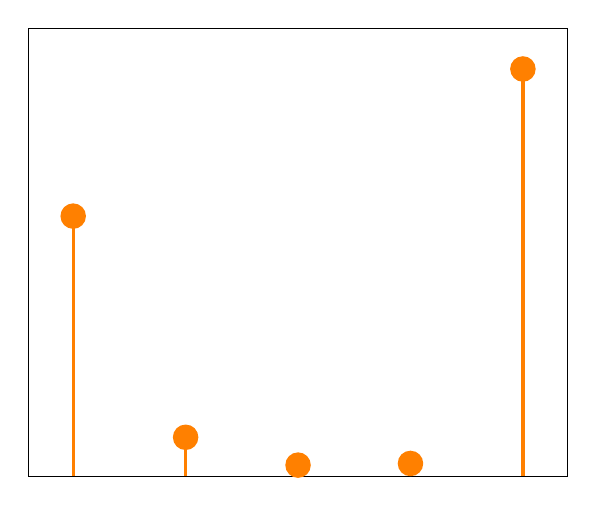
\begin{tikzpicture}background rectangle/.style={fill=white}, show background rectangle
					\begin{axis}[
						area style,
						axis background/.style={fill=white},
						ymin=0,
						ytick=\empty,
						xtick=\empty
					]
						\addplot+[ycomb, orange, mark=*, mark options={scale=2, fill=orange}, very thick] plot coordinates {
							(-8, 3623)
							(-7, 546)
							(-6, 159)
							(-5, 182)
							(-4, 5670)
						};
					\end{axis}
				\end{tikzpicture}
			}
		};
		\path (image) + (-.33, 1.66) node (segment_hist_5) {
			\resizebox{.75cm}{.75cm}{
				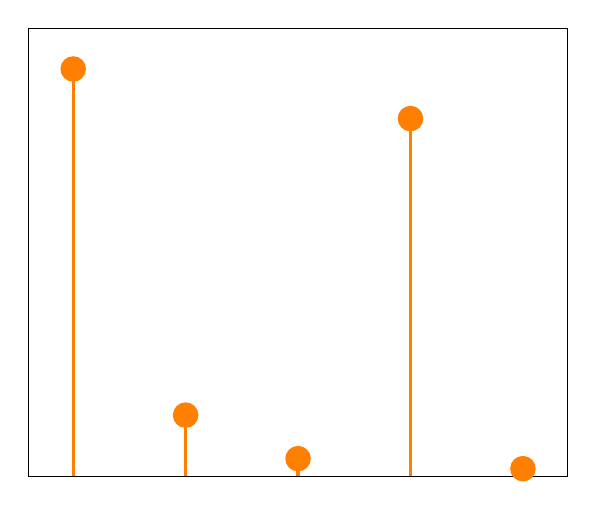
\begin{tikzpicture}background rectangle/.style={fill=white}, show background rectangle
					\begin{axis}[
						area style,
						axis background/.style={fill=white},
						ymin=0,
						ytick=\empty,
						xtick=\empty
					]
						\addplot+[ycomb, orange, mark=*, mark options={scale=2, fill=orange}, very thick] plot coordinates {
							(-8, 3623)
							(-7, 546)
							(-6, 159)
							(-5, 3182)
							(-4, 70)
						};
					\end{axis}
				\end{tikzpicture}
			}
		};
		\path (image) + (1.66, 1) node (segment_hist_6) {
			\resizebox{.75cm}{.75cm}{
				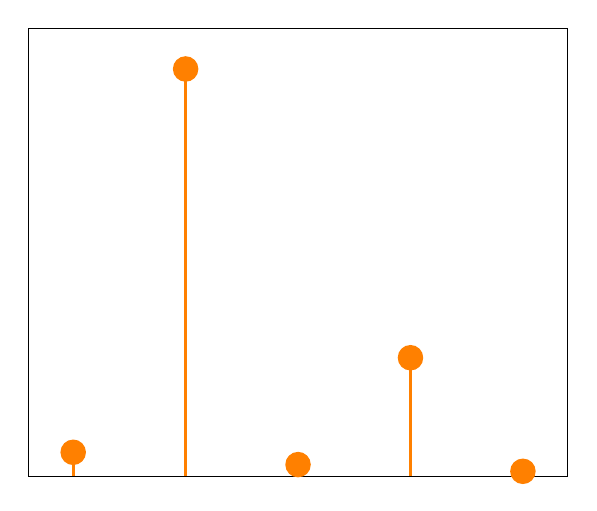
\begin{tikzpicture}background rectangle/.style={fill=white}, show background rectangle
					\begin{axis}[
						area style,
						axis background/.style={fill=white},
						ymin=0,
						ytick=\empty,
						xtick=\empty
					]
						\addplot+[ycomb, orange, mark=*, mark options={scale=2, fill=orange}, very thick] plot coordinates {
							(-8, 323)
							(-7, 5426)
							(-6, 159)
							(-5, 1582)
							(-4, 70)
						};
					\end{axis}
				\end{tikzpicture}
			}
		};
		\path (image) + (1.16, -.33) node (segment_hist_7) {
			\resizebox{.75cm}{.75cm}{
				\begin{tikzpicture}background rectangle/.style={fill=white}, show background rectangle
					\begin{axis}[
						area style,
						axis background/.style={fill=white},
						ymin=0,
						ytick=\empty,
						xtick=\empty
					]
						\addplot+[ycomb, orange, mark=*, mark options={scale=2, fill=orange}, very thick] plot coordinates {
							(-8, 23)
							(-7, 5456)
							(-6, 159)
							(-5, 182)
							(-4, 70)
						};
					\end{axis}
				\end{tikzpicture}
			}
		};
		\path (image) node (segment_hist_8) {
			\resizebox{.75cm}{.75cm}{
				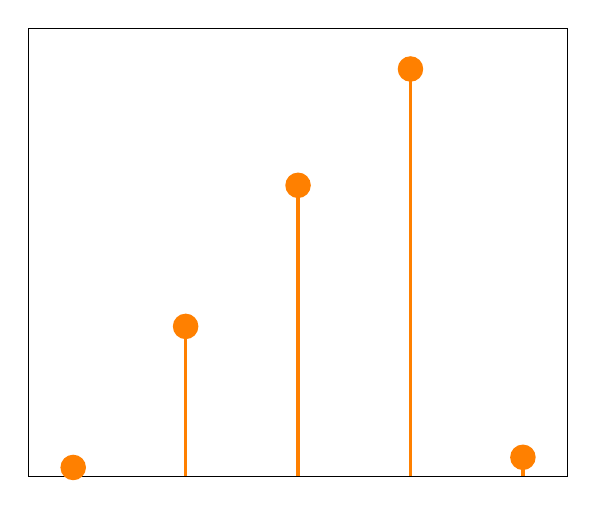
\begin{tikzpicture}background rectangle/.style={fill=white}, show background rectangle
					\begin{axis}[
						area style,
						axis background/.style={fill=white},
						ymin=0,
						ytick=\empty,
						xtick=\empty
					]
						\addplot+[ycomb, orange, mark=*, mark options={scale=2, fill=orange}, very thick] plot coordinates {
							(-8, 33)
							(-7, 546)
							(-6, 1059)
							(-5, 1482)
							(-4, 70)
						};
					\end{axis}
				\end{tikzpicture}
			}
		};
		\path (image) + (-1, .66) node (segment_hist_9) {
			\resizebox{.75cm}{.75cm}{
				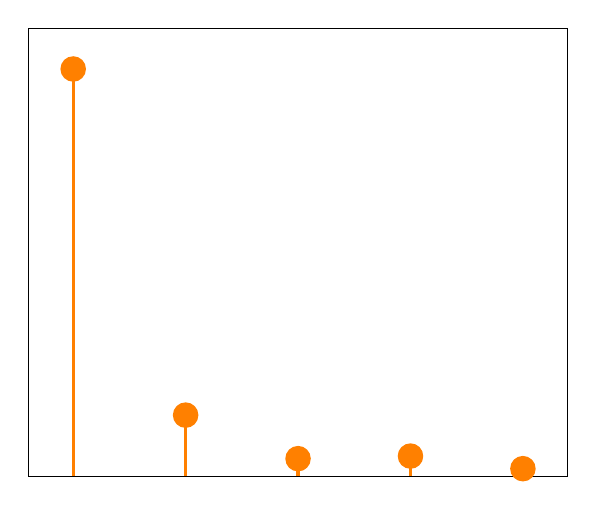
\begin{tikzpicture}background rectangle/.style={fill=white}, show background rectangle
					\begin{axis}[
						area style,
						axis background/.style={fill=white},
						ymin=0,
						ytick=\empty,
						xtick=\empty
					]
						\addplot+[ycomb, orange, mark=*, mark options={scale=2, fill=orange}, very thick] plot coordinates {
							(-8, 3623)
							(-7, 546)
							(-6, 159)
							(-5, 182)
							(-4, 70)
						};
					\end{axis}
				\end{tikzpicture}
			}
        };
	\end{tikzpicture}
\end{document}
